\begin{frame}{Konstrukcija pravokotnice}
	\begin{columns}
		\begin{column}{0.55\textwidth}
	\begin{itemize}[<+->]
		\item Dana sta premica \(p\) in točka \(T\).
		\item Nariši lok \(k\) s središčem v \(T\).
		\item Lok \(k\) seče premico \(p\) v točkah \(A\) in \(B\).
		\item Nariši lok \(m\) s središčem v \(A\).
		\item Nariši lok \(n\) s središčem v \(B\) in z enakim polmerom.
		\item Loka se sečeta v točki \(C\).
		\item Premica \(TC\) je pravokotna na \(p\).
	\end{itemize}
	\end{column}
	\begin{column}{0.45\textwidth}
		\centering
	\only{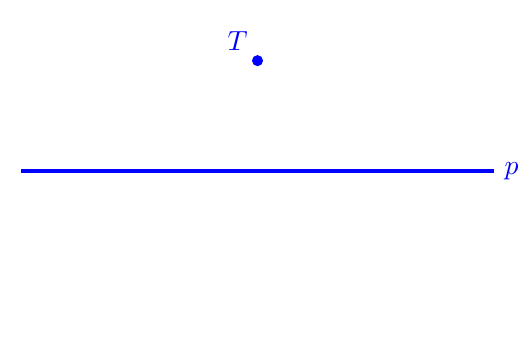
\includegraphics[width=50mm]{slike/fig-1.png}}<1>
	\only{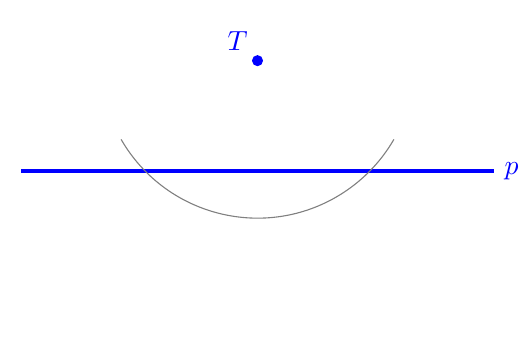
\includegraphics[width=50mm]{slike/fig-2.png}}<2>
	\only{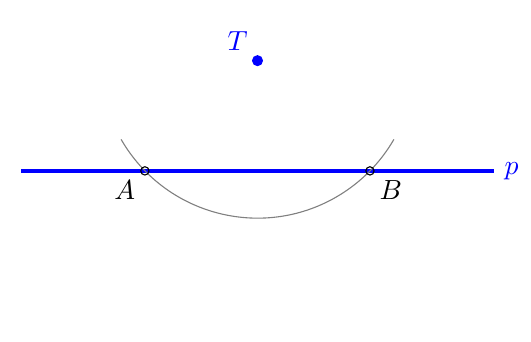
\includegraphics[width=50mm]{slike/fig-3.png}}<3>
	\only{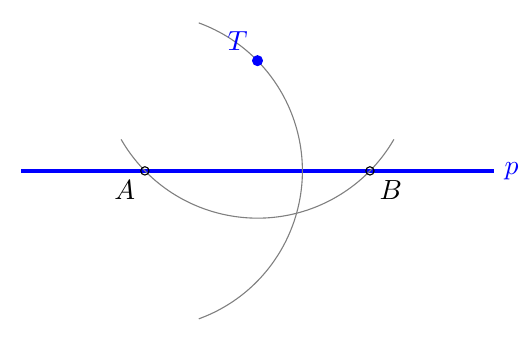
\includegraphics[width=50mm]{slike/fig-4.png}}<4>
	\only{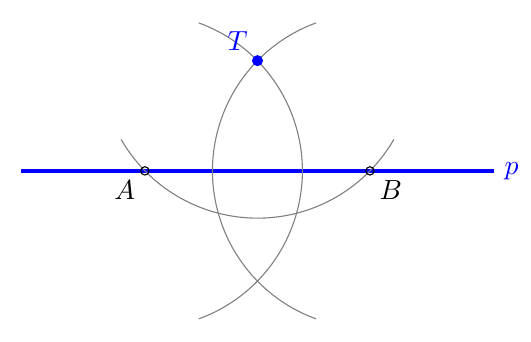
\includegraphics[width=50mm]{slike/fig-5.png}}<5>
	\only{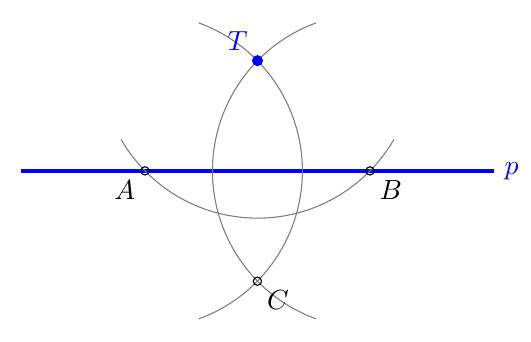
\includegraphics[width=50mm]{slike/fig-6.png}}<6>
	\only{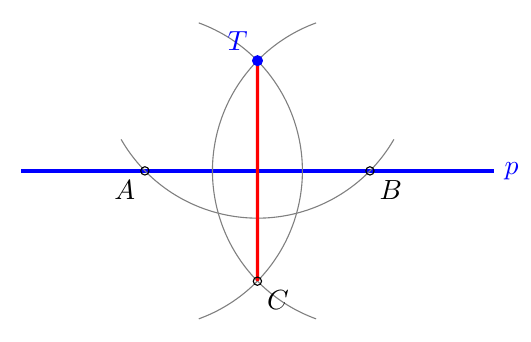
\includegraphics[width=50mm]{slike/fig-7.png}}<7>
	\end{column}
	\end{columns}
\end{frame}
